\documentclass[10pt,a4paper]{article}
\usepackage[utf8]{inputenc}
\usepackage[german]{babel}
\usepackage{amsmath}
\usepackage{amsfonts}
\usepackage{amssymb}
\usepackage[left=2cm,right=2cm,top=2cm,bottom=2cm]{geometry}

\usepackage{graphicx}

\author{Christian Bespin \and Christopher Deutsch}
\title{Übungsblatt 1: Numerische Methoden der Physik}
\begin{document}
\maketitle

\section{Madelung-Konstante des NaCl-Kristalls}
\subsection{Physikalischer Hintergrund}
In einem Kristallgitter sind die Ionen durch elektrostatische Wechselwirkung
untereinander an den Kristall gebunden. Uns interessiert die durchschnittliche
potentielle Energie eines dieser Ionen (wird mit dem Index $i$ bezeichnet).
Diese entsteht in erster Näherung aus der Überlagerung der Coulomb-Potentiale
der Punktladungen im Kristallgefüge
(werden mit dem Index $j$ bezeichnet). Die Ladungszahl des jeweiligen Ions sei $z$
und $r_{ij}$ ist der Abstand des betrachteten Ionenpaars. Wir summieren für
jedes Ion des Kristalls (mit Ausnahme des $i$-Ions, da dessen Potential auf sich
selbst keinen Einfluss hat) den Beitrag zum Potential:

\begin{align}
\label{EPot}
E_G = \sum_{j\atop i \neq j} \frac{1}{4 \pi \epsilon_0}
\frac{z_i e \cdot z_j e}{r_{ij}}
\end{align}
Erweitern der Gleichung (\ref{EPot}) mit dem Gitterabstand $a$ und
Zusammenfassen des Faktors in die durchschnittliche Energie eines Ionenpaars
$E_P$ mit Abstand $a$ ergibt:

\begin{align}
E_G = \frac{1}{4 \pi \epsilon_0} \frac{e^2}{a} \sum_{j\atop i \neq j}
\frac{z_i z_j}{r_{ij}/a} = E_P \sum_{j\atop i \neq j} \frac{z_i z_j}{r_{ij}/a}
\end{align}
Schließlich wird die Geometrie des Kristalls in der Madelung-Konstante
zusammengefasst:

\begin{align}
\label{Madelungkonstante}
\alpha = \frac{E_G}{E_P} = \sum_{j\atop i \neq j} \frac{z_i z_j}{r_{ij}/a}
\end{align}
Dabei ist $r_{ij}/a$ der mit der Gitterkonstanten normalisierte Abstand der Ionen,
welcher im Folgenden ausschließlich für Längen verwendet wird.

\subsection{Algorithmus im 3-dimensionalen Fall}
\subsubsection{Struktur von Natriumchlorid}

Die nächsten Nachbarn eines jeden Ions sind sechs Ionen entgegengesetzter
Ladung. Diese Ionen befinden sich an den Eckpunkten eines regelmäßigen
Oktaeders. Dadurch kann das Vorzeichen der Ladung an der Gitterstelle
$\mathbf{r} = \left( x,y,z \right)$ durch:
\begin{align}
\mathrm{sgn}\left(z(\mathbf{r})\right) = \pm \left( -1 \right)^{x+y+z}
\end{align}
berechnet werden. Dabei wird das Vorzeichen so gewählt, dass dies mit der Ladung
des Ion im Zentrum des Würfels übereinstimmt (Na: $+$; Cl: $-$). Diese Tatsache
äußert sich auch darin, dass das Vorzeichen der Madelung-Konstante vom
betrachteten Ion abhängt (generell: $\alpha_{Na} = - \alpha_{Cl}$).
\subsubsection{Probleme der naiven Methode}

Zunächst wurde die naive Implementierung analog zur mathematischen Beschreibung
getestet. Dabei wurde die Madelung-Konstante für einen Würfel analog zu
Gl. (\ref{Madelungkonstante}), über sukzessive Erweiterung des Würfels um eine
Schale berechnet. Es fällt schnell die schlechte Konvergenz auf, die sich
physikalisch darin manifestiert, dass der Kristall, beim einfachen Erweitern
mit einer Hülle, nicht elektrisch neutral bleibt. Dieses Problem wurde von Evjen
\cite{Evjen} gelöst, indem er den Kristall in elektrisch neutrale Elementarzellen
aufteilt, dessen Ladung wie in Abbildung \ref{skalierungsgrafik3d} gewichtet
werden. In der Summe über alle Elementarzellen eines Würfels, läuft dies darauf
hinaus, dass die Ecken, Kanten, Seitenflächen des Würfels mit $\frac{1}{8}$,
$\frac{1}{4}$ bzw. $\frac{1}{2}$ gewichtet werden.

\subsubsection{Beschreibung}

Zur Berechnung legen wir den Ursprung des Koordinatensystems in den Mittelpunkt des
Würfels und betrachten eine Ausdehnung von $-m$ bis $m$.
Wir berechnen die Madelungkonstante sukzessiv, indem wir jeder Stirnfläche eine Lage
hinzufügen, wodurch die Kantenlänge des Würfels um $2$ zunimmt (Zeile XX).\\
Die einzelnen Ladungen werden nach der Methode von
Evjens \cite{Evjen} unterschiedlich gewichtet, wodurch, wie im nächsten Absatz genauer
erläutert, eine gute Konvergenz des Algorithmus folgt. Dazu werden die Ladungen im
Inneren voll gewichtet, die Ladungen auf der Würfeloberfläche jedoch nicht. Wie in
Abbildung \ref{skalierungsgrafik3d} zu sehen gehen die Ladungen auf den Seitenflächen mit
dem Faktor $1/2$, die an den Kanten mit dem Faktor $1/4$ und die an den Ecken mit Faktor
$1/8$ ein. (Dies ist darin begründet, dass bei Aneinanderreihung mehrerer Würfel diese
Ladungen entsprechend öfter vorkämen; es berühren sich immer zwei Flächen, vier Kanten
und acht Ecken.)\\
Wir gehen in jedem Schleifendurchlauf davon aus, dass aktuell die äußerste Schale berechnet
wird und summieren so zunächst nur über die gewichteten Ladungen (Variable \texttt{sum}).
Den zu voller Gewichtung fehlenden Anteil summieren wir in jedem Schleifendurchlauf in der Variable
\texttt{rest} auf. Falls die Abbruchbedingung noch nicht erfüllt ist, wird diese zur
Gesamtsumme addiert, denn dann wurde im vorherigen Schleifendurchlauf noch nicht die
äußerste Schale betrachtet und alle Ladungen müssen voll gewichtet werden. Diese Methode
wurde gewählt, um mithilfe von \texttt{rest} den mit jeder Vergrößerung des Würfels
hinzukommenden Beitrag auswerten zu können und ein sinnvolles Abbruchkriterium zu definieren.\\

\begin{figure}[h]
	\centering
	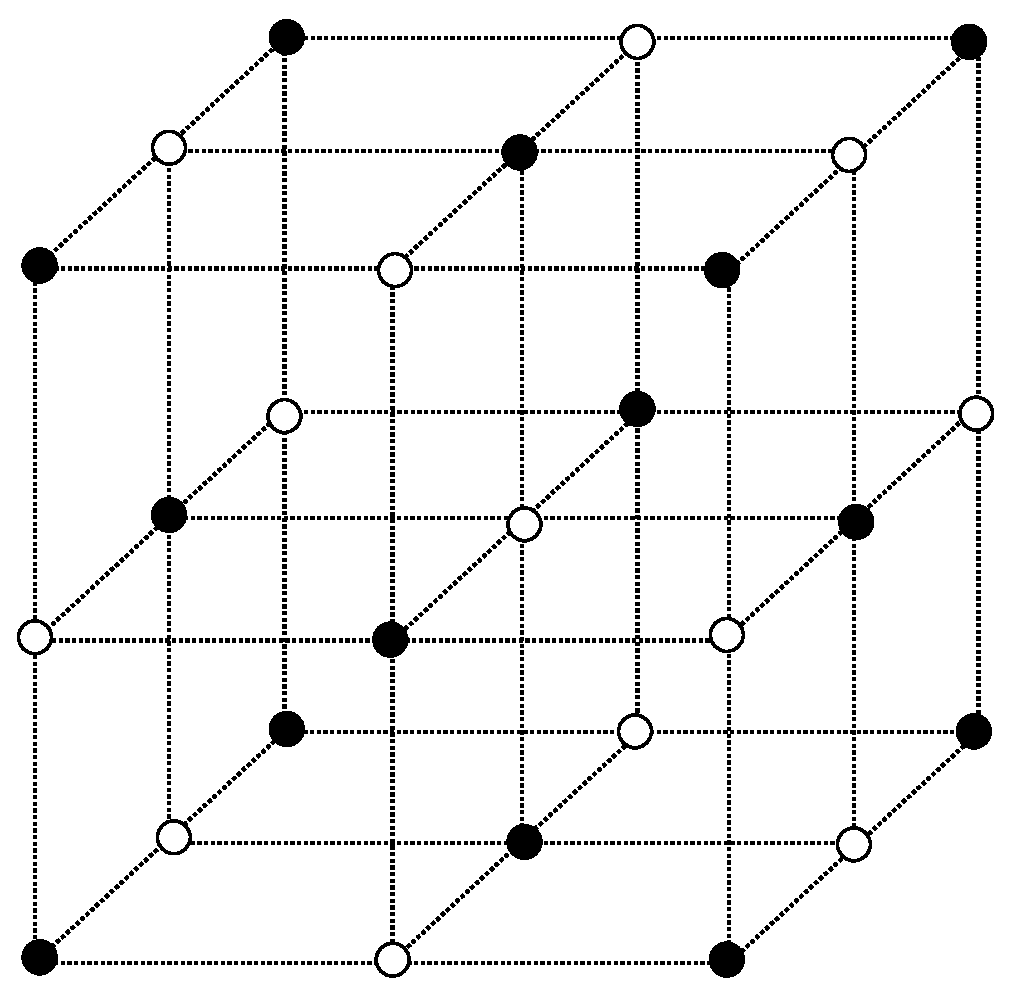
\includegraphics[scale = 0.4]{./figures/wuerfel.eps}
	\caption{neutrale Elementarzelle nach Evjen}
	\label{skalierungsgrafik3d}
\end{figure}
	

\subsubsection{Konvergenz}

\begin{itemize}
\item erkläre physikalischen Hintergrund für die bessere Konvergenz der Evjen
Methode
\item das Potential einer neutralen Elementarzelle fällt schneller ab als das
einer geladenen
\end{itemize}

\begin{table}[h]
\centering
\begin{tabular}{c|c|c}
\rule[-1ex]{0pt}{2.5ex} $n$ & $\alpha$ & $\delta$ \\ 
\hline 
\rule[-1ex]{0pt}{2.5ex} $4$ & $1.747721109631$ & $8.96\cdot10^{-5}$ \\ 
\hline 
\rule[-1ex]{0pt}{2.5ex} $8$ & $1.747574381726$ & $5.60\cdot10^{-6}$ \\ 
\hline 
\rule[-1ex]{0pt}{2.5ex} $20$ & $1.747564845218$ & $1.42\cdot10^{-7}$ \\ 
\hline 
\rule[-1ex]{0pt}{2.5ex} $50$ & $1.747564601048$ & $3.67\cdot10^{-9}$ \\ 
\hline 
\rule[-1ex]{0pt}{2.5ex} $100$ & $1.747564595034$ & $2.30\cdot10^{-10}$ \\ 
\end{tabular} 
\caption{Konvergenz}
\end{table}

\subsection{Algorithmus im 2-dimensionalen Fall}
\subsubsection{Beschreibung}
Die Methode von Evjen zur Gewichtung der Ladung ist leicht vom 3-Dimensionalen
in das 2-Dimensionale zu übertragen, denn es ist leicht zu sehen, dass um elektrische
Neutralität einer Elementarzelle zu erreichen, die Ecken mit $\frac{1}{4}$ und die Kanten mit
$\frac{1}{2}$ gewichtet werden müssen (Abbildung \ref{skalierungsgrafik2d}).

\begin{figure}[h]
	\centering
	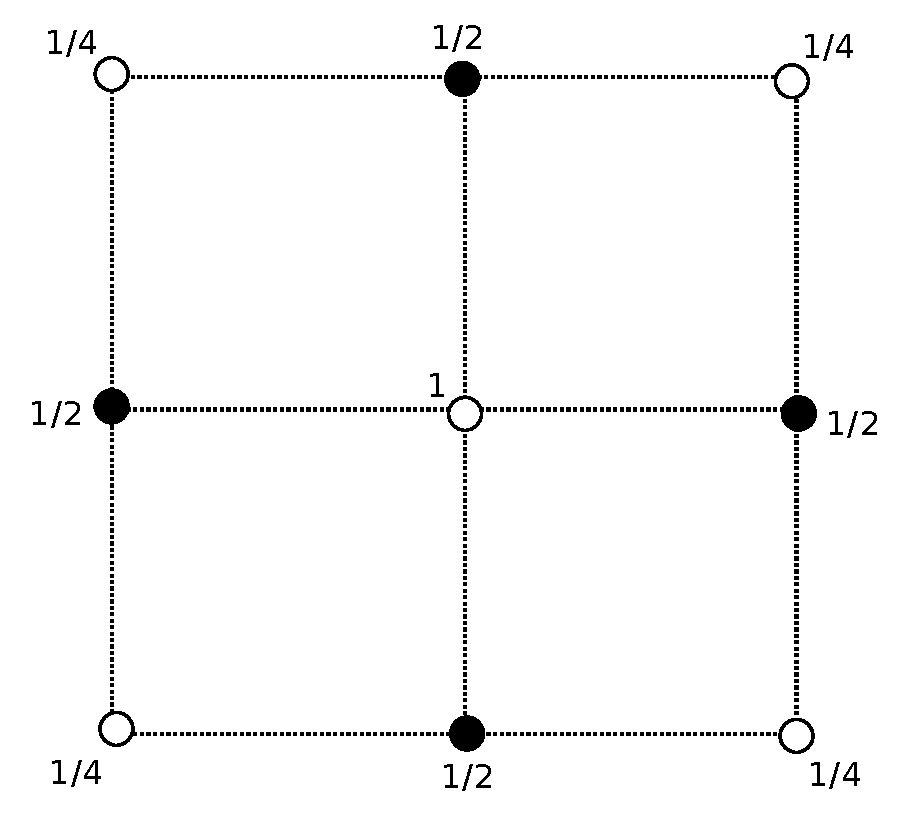
\includegraphics[scale = 0.4]{./figures/quadrat.eps}
	\caption{neutrale Elementarzelle in zwei Dimensionen}
	\label{skalierungsgrafik2d}
\end{figure}

\subsubsection{Konvergenz}

Wie gut konvergiert der 2-dimensionale Algorithmus.

\subsection{Fazit}

Verwendeter Literaturwert $\alpha_{NaCl} = 1.7475646946331822$ \cite{Sakamoto} .


\begin{thebibliography}{9}

\bibitem{Evjen}
Evjen, H. M.
\emph{On the Stability of Certain Heteropolar Crystals},
Physical Review Letters \textbf{39},
675-687 (1932)

\bibitem{Sakamoto}
Sakamoto, Y.
\emph{Madelung Constants of Simple Crystals Expressed in Terms of Born's Basic
Potentials of 15 Figures},
The Journal of Chemical Physics \textbf{28},
164 (1958)

\end{thebibliography}

\end{document}
